\chapter{Rotation I: kinematics, torque and statics}\label{ch:rot1}

Everything so far treated bodies as points. Real objects have extent ---
they spin, they lean, they stay put under balanced torques. The good news
is that rotation is a translation of every idea in the book so far:
figure~\ref{fig:dict} is the dictionary, and it never lies.

\begin{figure}[htbp]\centering
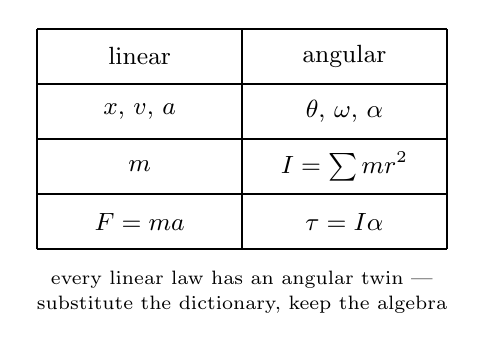
\begin{tikzpicture}[font=\small]
\draw[thick] (0,0) grid[xstep=2.6,ystep=0.7] (5.2,2.8);
\node at (1.3,2.45) {linear};\node at (3.9,2.45) {angular};
\node at (1.3,1.75) {$x$, $v$, $a$};\node at (3.9,1.75) {$\theta$, $\omega$, $\alpha$};
\node at (1.3,1.05) {$m$};\node at (3.9,1.05) {$I=\sum mr^{2}$};
\node at (1.3,0.35) {$F=ma$};\node at (3.9,0.35) {$\tau=I\alpha$};
\node[align=center] at (2.6,-0.55) {\scriptsize every linear law has an angular twin ---\\[-2pt]\scriptsize substitute the dictionary, keep the algebra};
\end{tikzpicture}

\caption{The linear--angular dictionary. Every equation in this chapter is
a ch1--ch2 equation with the entries swapped.}
\label{fig:dict}
\end{figure}

\section{Angular variables}\label{sec:rot-kin}

$\theta$ in radians, $\omega=\dot\theta$, $\alpha=\dot\omega$ --- and the
same constant-acceleration formulas of \S1.3 carry over verbatim:
$\omega=\omega_0+\alpha t$, $\theta=\theta_0+\omega_0t+\tfrac12\alpha t^{2}$,
$\omega^{2}=\omega_0^{2}+2\alpha\Delta\theta$. The rim variables are the
bridge: $v=\omega r$, $a_{\rm tan}=\alpha r$.

\section{Rolling kinematics: the no-slip constraint}\label{sec:rot-noslip}

A wheel rolling without slipping has $v_{\rm cm}=\omega r$ --- the contact
point is instantaneously at rest while the top moves at $2v$
(figure~\ref{fig:rolling}). The constraint is \emph{kinematic}, not
energetic: static friction enforces it without doing work, which is why
rolling races (ch6) are energy problems.

\begin{figure}[htbp]\centering
\begin{tikzpicture}[scale=1.0,force/.style={->,thick,accent}]
\draw[thick] (-0.5,0) -- (4.5,0);
\draw[thick] (2,1) circle (1);
\fill (2,1) circle (0.04) node[above left=-2pt,font=\scriptsize]{C};
\draw[force] (2,1) -- (3.3,1) node[right,font=\scriptsize]{$v$};
\draw[force] (2,2) -- (4.6,2) node[right,font=\scriptsize]{top: $2v$};
\draw[force] (2,0) -- (1.3,0) node[below,font=\scriptsize]{contact: $0$};
\draw[force] (3,1) -- (3.9,1.7) node[right,font=\scriptsize]{};
\node[font=\scriptsize] at (4.0,0.4) {$v=\omega r$ no-slip};
\draw[->,dashed] (2.6,1.4) arc (30:-60:0.55);
\node[font=\scriptsize] at (3.2,1.55) {$\omega$};
\end{tikzpicture}

\caption{Velocity field of a rolling wheel: centre at $v$, top at $2v$,
contact at $0$. Notice the contact point is a usable pivot for one
instant --- the seed of the instantaneous-axis trick.}
\label{fig:rolling}
\end{figure}

\section{Torque: force's lever-arm price}\label{sec:rot-torque}

\begin{equation}
  \boldsymbol\tau=\mathbf r\times\mathbf F,\qquad
  \tau=rF\sin\phi=\ell F,\label{eq:tau}
\end{equation}
where $\ell$ is the \emph{lever arm}\index{lever arm}: the perpendicular
distance from the pivot to the force's line of action
(figure~\ref{fig:torque}). Convention in this book: counterclockwise
positive. Torque is the quantity the door handle sells --- same force,
longer $\ell$, more angular acceleration.

\begin{figure}[htbp]\centering
\begin{tikzpicture}[scale=1.1,force/.style={->,thick,accent}]
\fill (0,0) circle (0.05) node[below left,font=\scriptsize]{pivot};
\draw[thick] (0,0) -- (3.5,0.9);
\draw[force] (3.5,0.9) -- (4.2,2.2) node[right,font=\scriptsize]{$\mathbf F$};
\draw[dashed] (0,0) -- (3.97,1.35);
\draw[dashed,amber] (0,0) -- (2.9,2.1) node[midway,above,font=\scriptsize]{$\ell$};
\draw[thick,amber] (2.9,2.1) -- (4.0,2.24);
\node[font=\scriptsize] at (1.7,0.7) {$\mathbf r$};
\node[font=\scriptsize,align=left] at (5.0,0.3) {$\tau=rF\sin\phi$\\$=\ell F$};
\draw[->,dashed] (0.8,0.35) arc (15:40:0.9);
\node[font=\scriptsize] at (1.15,0.75) {$\phi$};
\end{tikzpicture}

\caption{Torque geometry: $\tau=rF\sin\phi$, equivalently $\ell F$ with the
lever arm $\ell$. Notice only the perpendicular component of $\mathbf F$
pays.}
\label{fig:torque}
\end{figure}

\section{Moment of inertia: mass with an $r^{2}$ tax}\label{sec:rot-i}

\begin{equation}
  I=\sum_i m_ir_i^{2}\;\xrightarrow{\ \text{continuous}\ }\;
  I=\int r^{2}\,dm.\label{eq:moi}
\end{equation}
The $r^{2}$ is the whole story: mass near the axis is cheap, mass at the
rim is expensive --- a hoop resists twice as hard per kilogram as a disk.
Two theorems do most of the work: the \emph{parallel-axis} shift
$I=I_{\rm cm}+Md^{2}$, and the \emph{perpendicular-axis}
$I_z=I_x+I_y$ for flat laminas.

\begin{example}[$I$ of a rod and a disk by direct integration]\label{ex:moi}
Compute $I$ about the centre for (a) a uniform rod of length $L$, (b) a
uniform disk of radius $R$.
\par\smallskip
\textbf{Strategy.} Slice into rings/strips where $r$ is constant; the
integral is bookkeeping, not calculus difficulty.
\begin{solution}
(a) Rod: $dm=\lambda dx$ with $\lambda=M/L$:
$I=\int_{-L/2}^{L/2}x^{2}\lambda\,dx=\lambda\frac{L^{3}}{12}
=\frac{1}{12}ML^{2}$.
(b) Disk: rings of mass $dm=\sigma\,2\pi r\,dr$, all points at the same
$r$: $I=\int_0^{R}r^{2}\sigma2\pi r\,dr
=2\pi\sigma R^{4}/4=\frac{1}{2}MR^{2}$ using
$M=\sigma\pi R^{2}$. \checkmark
\end{solution}
\end{example}

\begin{figure}[htbp]\centering
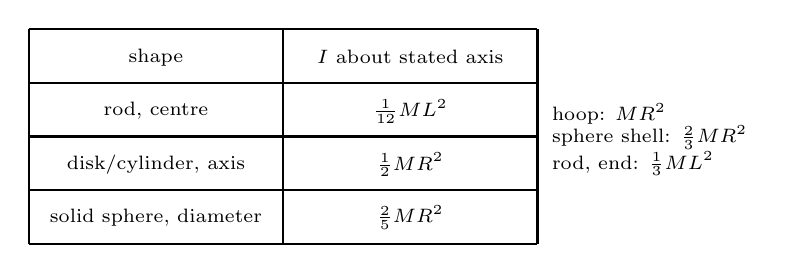
\begin{tikzpicture}[font=\scriptsize,scale=0.95]
\draw[thick] (0,0) grid[xstep=3.4,ystep=0.72] (6.8,2.88);
\node at (1.7,2.5) {shape};\node at (5.1,2.5) {$I$ about stated axis};
\node at (1.7,1.78) {rod, centre};\node at (5.1,1.78) {$\frac{1}{12}ML^{2}$};
\node at (1.7,1.06) {disk/cylinder, axis};\node at (5.1,1.06) {$\frac{1}{2}MR^{2}$};
\node at (1.7,0.36) {solid sphere, diameter};\node at (5.1,0.36) {$\frac{2}{5}MR^{2}$};
\node[align=left] at (8.3,1.4) {hoop: $MR^{2}$\\sphere shell: $\frac{2}{3}MR^{2}$\\rod, end: $\frac{1}{3}ML^{2}$};
\end{tikzpicture}

\caption{The six standard moments. Notice the coefficient tracks how far
mass sits from the axis --- the rod's $1/12$, the disk's $1/2$, the
hoop's $1$.}
\label{fig:itable}
\end{figure}

\begin{lstlisting}[language=Python,caption={\texttt{code/ch05\_inertia\_integrator.py} --- grid quadrature vs analytic $I$; the parallel-axis term on display.},label={lst:moi}]
s += r*r * r*dr*dth   # r^2 * dA, dA = r dr dth
\end{lstlisting}

Output of a real run:
\begin{lstlisting}[numbers=none]
rectangle 2.0x1.0: numeric I=0.8333, exact=0.8333, err=0.00%
  per unit mass: I/M=0.4167 vs (a^2+b^2)/12=0.4167
disk R=1.0: numeric I=1.5708, exact=1.5708, err=0.00%
  per unit mass: I/M=0.5000 vs R^2/2=0.5000
disk about rim: I=4.7124 = I_cm + M R^2 (1.5708 + 3.1416); ratio to I_cm = 3.00
\end{lstlisting}

Notice the last line: spinning a disk about a point on its rim costs
\emph{three times} the centre-axis moment --- the $Md^{2}$ term, not a
numerical artifact.

\section{$\tau=I\alpha$: the massive pulley}\label{sec:rot-tia}

With a real pulley the rope's two sides can't share a tension --- the
difference is what spins the wheel (figure~\ref{fig:pulley}).

\begin{figure}[htbp]\centering
\begin{tikzpicture}[scale=1.0,force/.style={->,thick,accent}]
\draw[thick] (-1.5,3.2) -- (1.5,3.2);
\draw[fill=gray!30] (0,3.2) circle (0.4);
\fill (0,3.2) circle (0.03);
\node[font=\scriptsize] at (0,3.85) {$I=\tfrac12MR^{2}$};
\draw (-0.4,3.2) -- (-0.4,1.2); \draw (0.4,3.2) -- (0.4,0.4);
\filldraw[fill=gray!20] (-0.75,0.7) rectangle (-0.05,1.2);
\node[font=\scriptsize] at (-0.4,0.95) {$m_1$};
\filldraw[fill=gray!20] (0.05,0.0) rectangle (0.75,0.4);
\node[font=\scriptsize] at (0.4,0.2) {$m_2$};
\draw[force] (-0.4,0.7) -- (-0.4,-0.15) node[below,font=\scriptsize]{$m_1g$};
\draw[force] (-0.4,1.2) -- (-0.4,2.0) node[above,font=\scriptsize]{$T_1$};
\draw[force] (0.4,0.0) -- (0.4,-0.85) node[below,font=\scriptsize]{$m_2g$};
\draw[force] (0.4,0.4) -- (0.4,1.3) node[above,font=\scriptsize]{$T_2$};
\node[font=\scriptsize,align=left] at (2.3,1.2) {$T_1\neq T_2$:\\the difference\\spins the pulley};
\end{tikzpicture}

\caption{The massive pulley's three-body problem: two hanging FBDs plus
$\sum\tau=I\alpha$ on the wheel. The tension \emph{difference} does the
spinning.}
\label{fig:pulley}
\end{figure}

\begin{example}[Atwood with a massive pulley]\label{ex:mpulley}
Repeat example 2.1's Atwood ($m_1=3$, $m_2=5$\,kg) with a pulley of mass
$M=4$\,kg, radius $R$, modeled as a disk ($I=\tfrac12MR^{2}$).
\par\smallskip
\textbf{Strategy.} Three equations: two translations plus one rotation.
Constraint: $\alpha=a/R$ (no slip on the rim).
\begin{solution}
$m_2g-T_2=m_2a$, $T_1-m_1g=m_1a$, and
$(T_2-T_1)R=I\alpha=\tfrac12MR^{2}\cdot a/R \Rightarrow T_2-T_1=\tfrac12Ma$.
Adding all three:
\[
  a=\frac{(m_2-m_1)g}{m_1+m_2+M/2}
   =\frac{2\times9.8}{3+5+2}=1.96\,\mathrm{m/s^{2}},
\]
down from $2.45$ --- the pulley acts like an extra $2$\,kg of inertia.
$T_1=35.3$\,N, $T_2=39.2$\,N: no longer equal, and their difference
$3.9$\,N is exactly $\tfrac12Ma$. \checkmark
\end{solution}
\end{example}

\begin{example}[Yo-yo unwinding]\label{ex:yoyo}
A yo-yo (disk, $I=\tfrac12mR^{2}$, string wrapped at radius $r$) falls
unwinding. Find its acceleration.
\par\smallskip
\textbf{Strategy.} Two equations: $mg-T=ma$ and $Tr=I\alpha$ with
$\alpha=a/r$.
\begin{solution}
$T=I a/r^{2}=\tfrac12mR^{2}a/r^{2}$, so
$a=\frac{g}{1+R^{2}/(2r^{2})}$. For $R/r=5$: $a=g/13.5=0.73$\,m/s$^{2}$
--- the rim-radius leverage makes it a slow fall. \checkmark
\end{solution}
\end{example}

\begin{exercise}[medium]
Find $a$ for the yo-yo when it's a hoop ($I=mR^{2}$) instead. (F=ma)
\end{exercise}

\section{Statics: two balances, one smart pivot}\label{sec:rot-static}

Static equilibrium needs $\sum\mathbf F=0$ \emph{and}
$\sum\boldsymbol\tau=0$ --- and the pivot for the second equation is
\emph{yours to choose}: put it where an unknown force acts and that force
disappears from the torque books. That single trick solves most of the
chapter's problems.

\begin{example}[Ladder minimum angle]\label{ex:ladder}
A uniform ladder of length $L$ leans at angle $\theta$ against a
frictionless wall (figure~\ref{fig:ladder}); the floor has $\mu_s$.
Minimum $\theta$ before slipping?
\par\smallskip
\textbf{Strategy.} $\sum F$: $N_2=f$, $N_1=mg$. Torque about the base
(kills $f$ and $N_1$): the wall's push at the top balances gravity at the
middle.
\begin{solution}
$N_2 L\sin\theta=mg\frac{L}{2}\cos\theta \Rightarrow
N_2=\frac{mg}{2\tan\theta}$. Slip when $f=N_2=\mu_sN_1=\mu_smg$:
$\tan\theta_{\min}=\frac{1}{2\mu_s}$. For $\mu_s=0.4$: $\theta_{\min}=
51.3^{\circ}$ --- below that, the wall can't push hard enough. \checkmark
\end{solution}
\end{example}

\begin{figure}[htbp]\centering
\begin{tikzpicture}[scale=1.0,force/.style={->,thick,accent}]
\draw[thick] (0,0) -- (0,4); \draw[thick] (0,0) -- (3.5,0);
\draw[very thick] (0,0.2) -- (2.6,3.8);
\fill (1.3,2.0) circle (0.06);
\draw[force] (1.3,2.0) -- (1.3,0.9) node[right,font=\scriptsize]{$mg$};
\draw[force] (0,0.2) -- (0.7,0.2) node[right,font=\scriptsize]{$f$};
\draw[force] (0,0.2) -- (0,0.95) node[above,font=\scriptsize]{$N_1$};
\draw[force] (2.6,3.8) -- (1.9,3.8) node[left,font=\scriptsize]{$N_2$};
\draw (0.55,0) arc (0:55:0.55); \node[font=\scriptsize] at (0.8,0.35) {$\theta$};
\node[font=\scriptsize,align=left] at (4.3,3.0) {smart pivot: base ---\\kills $f$ and $N_1$};
\end{tikzpicture}

\caption{Ladder FBD: frictionless wall means $N_2$ is purely horizontal;
taking torques about the base deletes both floor forces.}
\label{fig:ladder}
\end{figure}

\begin{exercise}[easy]
Where does a second person standing halfway up the ladder change the
minimum angle? Set up the new torque equation. (AP-C)
\end{exercise}

\begin{example}[Two-support beam]\label{ex:beam}
A uniform $8$\,kg, $5$\,m beam rests on supports at $x=1$ and $x=4$
(metres from the left end), with a $20$\,kg toolbox at $x=4.5$. Find each
support's force.
\par\smallskip
\textbf{Strategy.} $\sum F$ gives the sum; torque about one support kills
its unknown. Watch: the toolbox overhangs the right support.
\begin{solution}
$N_A+N_B=mg+Mg=78.4+196=274.4$\,N.
Torque about support $A$ (CCW$+$): the beam's weight acts at $x=2.5$
(1.5\,m right of $A$), the toolbox at $3.5$\,m right, $N_B$ at $3$\,m:
$3N_B=78.4\times1.5+196\times3.5=117.6+686$, so $N_B=267.9$\,N and
$N_A=6.5$\,N --- the left support nearly unloads: shift the toolbox a
little further and the beam tips. \checkmark
\end{solution}
\end{example}

\section{Rotational kinetic energy}\label{sec:rot-ke}

$K_{\rm rot}=\tfrac12I\omega^{2}$, and for rolling
$K=\tfrac12mv^{2}+\tfrac12I\omega^{2}$ --- the reason a hoop loses every
race down an incline: it pays the rotation tax with the largest per-mass
$I$ (chapter~6 races them properly).

\section{In engineering practice: torque specs}\label{sec:rot-eng}

Every bolt in a car has a printed torque spec --- this chapter's
$\tau=\ell F$ run as quality control: a $25$\,N\,m spec on a $0.25$\,m
wrench means exactly $100$\,N of hand force, and overtightening stretches
the bolt past its elastic range (book5's materials chapter has the yield
story). The statics side is how cranes stay up: $\sum\tau=0$ about the
outrigger line is the tip-over condition, which is why load charts shrink
with boom extension --- longer $\ell$, same budget.

\section{Common mistakes}\label{sec:rot-mistakes}

\begin{tripwire}[Lever arm vs point distance]
$\tau=\ell F$: $\ell$ is perpendicular distance to the \emph{line of
action}, not to the point of application along the body.
\end{tripwire}
\begin{tripwire}[Forgetting the pulley's inertia]
A massless pulley shares one $T$; a massive one doesn't --- drop the
$\tfrac12Ma$ term and the answer is too fast.
\end{tripwire}
\begin{tripwire}[Wrong parallel-axis shift]
$I=I_{\rm cm}+Md^{2}$ --- it's about the CM plus a shift, never between
two arbitrary axes.
\end{tripwire}
\begin{tripwire}[Bad torque origin]
Every force through the origin drops out. Pick the pivot at the unknown
you want gone, not at the centre because it looks official.
\end{tripwire}
\begin{tripwire}[Force balance alone in statics]
$\sum F=0$ admits a whole family of torques; the ladder needs
$\sum\tau=0$ too.
\end{tripwire}

\section{Summary}\label{sec:rot-summary}

\begin{table}[ht]\centering
\begin{tabularx}{\linewidth}{@{}lY@{}}
\toprule
\tablehead\thead{Idea} & \thead{One-line version}\\
\midrule
dictionary & $\theta/\omega/\alpha \leftrightarrow x/v/a$; same formulas \\
no-slip & $v_{\rm cm}=\omega r$; contact instant rest, top $2v$ \\
torque & $\tau=rF\sin\phi=\ell F$; CCW positive \\
moment of inertia & $I=\int r^{2}dm$; $1/12$, $1/2$, $2/5$ coefficients \\
dynamics & $\tau=I\alpha$; massive pulleys need $T_1\neq T_2$ \\
statics & $\sum F=0$ + $\sum\tau=0$; pivot at the unknown \\
rotational $K$ & $\tfrac12I\omega^{2}$; rolling pays both \\
\bottomrule
\end{tabularx}
\caption{Rotation-I cheat sheet.}
\label{tab:rotsummary}
\end{table}

\begin{wins}[Definition of done]
You can now: run the linear--angular dictionary; read a rolling wheel's
velocity field; compute lever arms and torques; integrate $I$ for simple
shapes and apply parallel axis; solve massive-pulley and yo-yo dynamics;
and set up statics with the smart-pivot trick.
\end{wins}

\chapternotes{%
The dictionary-first approach follows MIT 8.01SC weeks 6 and 10--11
\cite{ocw801} and AP Physics C unit 5 \cite{apced}. OpenStax College
Physics ch.~10, 12 \cite{openstax1} covers the same ground; the ladder and
pulley problems are Morin chs.~7--8 \cite{morin} classics. The I-table
coefficients are standard; the quadrature listing checks two of them
numerically.}

\begin{rulebox}[{Watch instead}]
\begin{enumerate}
\item \emph{Rotating Objects, Moment of Inertia, Rotational KE, Neutron
Stars} --- Walter Lewin, MIT 8.01x Lecture 19, 41:00,
\url{https://youtu.be/fDJeVR0o__w} --- \S\ref{sec:rot-i}--\S\ref{sec:rot-ke}
at full length (accessed 2026-10-11).
\item \emph{Angular motion variables} --- Khan Academy Physics, 12:50,
\url{https://youtu.be/garegCgMxxg} --- \S\ref{sec:rot-kin}--\S\ref{sec:rot-noslip}
worked quickly (accessed 2026-10-11).
\end{enumerate}
\end{rulebox}

\section*{Further reading}
\addcontentsline{toc}{section}{Further reading}

\begin{itemize}
\item MIT OpenCourseWare, \emph{8.01SC Classical Mechanics}, weeks 6,
10--11 --- rotation and statics with recitation solutions. At
\url{https://ocw.mit.edu}, course ``8.01SC'' (verified 2026-10-11).
\item OpenStax, \emph{College Physics 2e}, ch.~10 ``Rotational Motion''
and ch.~12 ``Statics'' --- free text at \url{https://openstax.org}
(verified 2026-10-11).
\item College Board, \emph{AP Physics C: Mechanics CED}, Unit 5 --- the
exam blueprint for rotation. At \url{https://apstudents.collegeboard.org}
(verified 2026-10-11).
\item D.~Morin, \emph{Introduction to Classical Mechanics}, chs.~7--8 ---
statics and rotation at the harder level; ISBN 978-0521876223.
\item The Physics Classroom, \emph{Rotational Motion} tutorials ---
readable remediation for \S\ref{sec:rot-kin}--\S\ref{sec:rot-static}, at
\url{https://www.physicsclassroom.com} (verified 2026-10-11).
\item Khan Academy, \emph{Moments, torque, and angular momentum} ---
drills matching the whole chapter, at
\url{https://www.khanacademy.org} under Science $\to$ Physics (verified
2026-10-11).
\end{itemize}

\section*{Additional exercises}
\addcontentsline{toc}{section}{Additional exercises}

\begin{exercise}[easy]
A wheel spins up to $1200$\,rpm in $4$\,s at constant $\alpha$. Find
$\alpha$ in $\mathrm{rad/s^{2}}$ and the angle turned. (AP-C)
\end{exercise}
\begin{exercise}[easy]
Identify the lever arm: a $0.5$\,m wrench at $60^{\circ}$ to a $100$\,N
force --- compute $\tau$ both as $rF\sin\phi$ and $\ell F$. (AP-C)
\end{exercise}
\begin{exercise}[easy]
Write down $I$ for a $2$\,kg, $0.3$\,m-radius disk about its axis and
about a rim point, citing the theorem used. (AP-C)
\end{exercise}
\begin{exercise}[easy]
A uniform beam of length $4$\,m is pinned at one end and carries a
$200$\,N load at its far end. What vertical force at the midpoint holds
it level (neglecting the beam's weight)? (F=ma)
\end{exercise}
\begin{exercise}[easy]
A see-saw: $30$\,kg child at $1.5$\,m left of the pivot balances a
$50$\,kg adult. Where does the adult sit? (F=ma)
\end{exercise}
\begin{exercise}[medium]
Massive-pulley Atwood: recompute example~\ref{ex:mpulley} with a hoop
pulley ($I=MR^{2}$) --- which way does $a$ move, and why? (F=ma classic)
\end{exercise}
\begin{exercise}[medium]
Redo example~\ref{ex:ladder} with a wall that has $\mu_s'=0.3$ of its
own. Does the wall friction help or hurt? (AP-C FR-style)
\end{exercise}
\begin{exercise}[medium]
A yo-yo hoop ($I=mR^{2}$, string at $r$) falls unwinding --- find $a$
and compare with example~\ref{ex:yoyo}. (F=ma)
\end{exercise}
\begin{exercise}[medium]
Composite body: a $0.5$\,m rod of mass $2$\,kg has a $1$\,kg,
$0.1$\,m-radius disk welded at one end (disk axis through the rod's end,
perpendicular). Find $I$ about the rod's other end. (AP-C)
\end{exercise}
\begin{exercise}[medium]
Sign-of-torque reasoning: a door pushed at its top vs its middle, same
force --- describe the angular acceleration ratio without computing.
(AP-C)
\end{exercise}
\begin{exercise}[medium]
Rolling preview: a hoop and a disk race down an incline from rest ---
predict the winner using only the $I$ coefficients, then verify with
energy ($v^{2}=\frac{2gh}{1+I/mr^{2}}$). (AP-C)
\end{exercise}
\begin{exercise}[medium]
A uniform $8$\,kg beam $5$\,m long rests on two supports at $x=1$ and
$x=4$ (metres). Find each reaction force. (F=ma)
\end{exercise}
\begin{exercise}[hard]
A uniform rod leans on a frictionless floor against a frictionless wall
and is released. Show it loses wall contact when
$\sin\theta=\frac{2}{3}\sin\theta_0$ --- use energy for speed and the CM's
horizontal acceleration for the contact condition. (USAPhO-style)
\end{exercise}
\begin{exercise}[hard]
A rod of length $L$ has density $\lambda(x)=\lambda_0(1+x/L)$. Find its
$I$ about the light end by direct integration, and its CM. (APhO-style)
\end{exercise}
\begin{exercise}[medium]
A sphere and a cylinder of the same $M$, $R$ roll (not slide) down the
same incline. Using $v^{2}=\frac{2gh}{1+I/mr^{2}}$, find the sphere's
speed advantage over the cylinder's at the bottom as a percentage.
(AP-C)
\end{exercise}
